%!TEX TS-program = pdflatexmk

% Copyright (c) 2018 - 2022, Martin Scheidt (ISC license)
% Permission to use, copy, modify, and/or distribute this file for any purpose with or without fee is hereby granted, provided that the above copyright notice and this permission notice appear in all copies.

\documentclass[border=2]{standalone}

\usepackage[dev]{tikz-trackschematic}

\begin{document}
  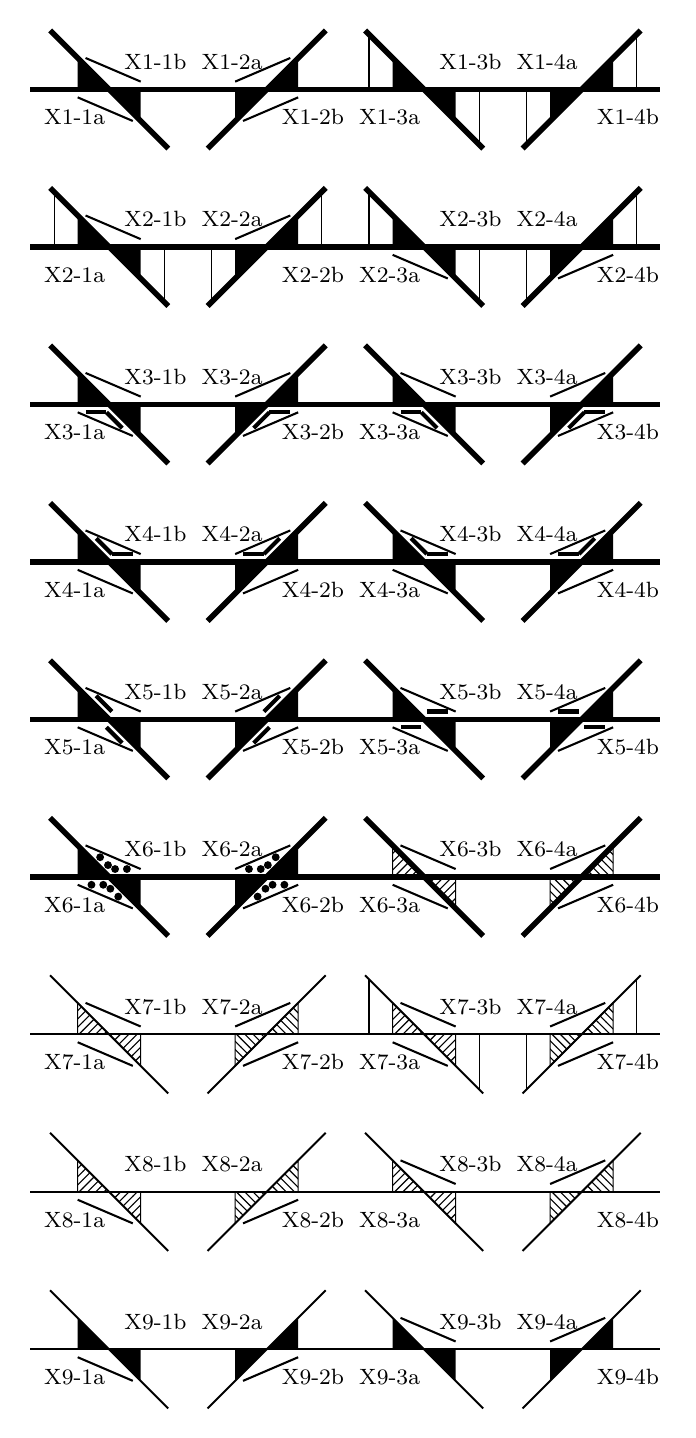
\begin{tikzpicture}
  
    \foreach \i in {1,2,...,9}{% base coordinate
      \coordinate (A\i) at ($(0,0) + 2*(0,-\i)$);% base coordinate
      \coordinate (B\i) at ($(8,0) + 2*(0,-\i)$);% base coordinate
    }

    \foreach \i in {1,2,...,6}{% draw main tracks on base coordinate
      \maintrack (A\i) --   (B\i);
    }

    \foreach \i in {7,8,...,9}{% draw secondary tracks on base coordinate
      \secondarytrack (A\i) --   (B\i);
    }

    \foreach \i in {1,2,...,9}{% coordinates for testing symbols
      \coordinate (X\i-1) at ($(1,0) + 2*(0,-\i)$);
      \coordinate (X\i-2) at ($(3,0) + 2*(0,-\i)$);
      \coordinate (X\i-3) at ($(5,0) + 2*(0,-\i)$);
      \coordinate (X\i-4) at ($(7,0) + 2*(0,-\i)$);
    }

    \foreach \i in {1,2,...,6}{% coordinates for testing symbols
      \maintrack (X\i-1) -- ++( 0.75,-0.75);
      \maintrack (X\i-1) -- ++(-0.75, 0.75);
      \maintrack (X\i-2) -- ++( 0.75, 0.75);
      \maintrack (X\i-2) -- ++(-0.75,-0.75);
      \maintrack (X\i-3) -- ++( 0.75,-0.75);
      \maintrack (X\i-3) -- ++(-0.75, 0.75);
      \maintrack (X\i-4) -- ++( 0.75, 0.75);
      \maintrack (X\i-4) -- ++(-0.75,-0.75);
    }

    \foreach \i in {7,8,...,9}{% coordinates for testing symbols
      \secondarytrack (X\i-1) -- ++( 0.75,-0.75);
      \secondarytrack (X\i-1) -- ++(-0.75, 0.75);
      \secondarytrack (X\i-2) -- ++( 0.75, 0.75);
      \secondarytrack (X\i-2) -- ++(-0.75,-0.75);
      \secondarytrack (X\i-3) -- ++( 0.75,-0.75);
      \secondarytrack (X\i-3) -- ++(-0.75, 0.75);
      \secondarytrack (X\i-4) -- ++( 0.75, 0.75);
      \secondarytrack (X\i-4) -- ++(-0.75,-0.75);
    }

    \slipturnout[branch=right] at (X1-1) label (X1-1a)(X1-1b);
    \slipturnout[branch=left ] at (X1-2) label (X1-2a)(X1-2b);
    \slipturnout[branch=right,slip=none,fouling point] at (X1-3) label (X1-3a)(X1-3b);
    \slipturnout[branch=left ,slip=none,fouling point] at (X1-4) label (X1-4a)(X1-4b);

    \slipturnout[branch=right,slip=left ,fouling point] at (X2-1) label (X2-1a)(X2-1b);
    \slipturnout[branch=left ,slip=left ,fouling point] at (X2-2) label (X2-2a)(X2-2b);
    \slipturnout[branch=right,slip=right,fouling point] at (X2-3) label (X2-3a)(X2-3b);
    \slipturnout[branch=left ,slip=right,fouling point] at (X2-4) label (X2-4a)(X2-4b);

    \slipturnout[branch=right,forward points=right,backward points=left] at (X3-1) label (X3-1a)(X3-1b);
    \slipturnout[branch=left ,forward points=right,backward points=left] at (X3-2) label (X3-2a)(X3-2b);
    \slipturnout[branch=right,forward points=right,backward points=left] at (X3-3) label (X3-3a)(X3-3b);
    \slipturnout[branch=left ,forward points=right,backward points=left] at (X3-4) label (X3-4a)(X3-4b);

    \slipturnout[branch=right,forward points=left,backward points=right] at (X4-1) label (X4-1a)(X4-1b);
    \slipturnout[branch=left ,forward points=left,backward points=right] at (X4-2) label (X4-2a)(X4-2b);
    \slipturnout[branch=right,forward points=left,backward points=right] at (X4-3) label (X4-3a)(X4-3b);
    \slipturnout[branch=left ,forward points=left,backward points=right] at (X4-4) label (X4-4a)(X4-4b);

    \slipturnout[branch=right,forward points=right,backward points=right] at (X5-1) label (X5-1a)(X5-1b);
    \slipturnout[branch=left ,forward points=left ,backward points=left] at (X5-2) label (X5-2a)(X5-2b);
    \slipturnout[branch=right,forward points=left ,backward points=left ] at (X5-3) label (X5-3a)(X5-3b);
    \slipturnout[branch=left ,forward points=right,backward points=right] at (X5-4) label (X5-4a)(X5-4b);

    \slipturnout[branch=right,forward points=moving,backward points=moving] at (X6-1) label (X6-1a)(X6-1b);
    \slipturnout[branch=left ,forward points=moving,backward points=moving] at (X6-2) label (X6-2a)(X6-2b);
    \slipturnout[branch=right,operation=manual] at (X6-3) label (X6-3a)(X6-3b);
    \slipturnout[branch=left ,operation=manual] at (X6-4) label (X6-4a)(X6-4b);

    \slipturnout[branch=right,operation=manual] at (X7-1) label (X7-1a)(X7-1b);
    \slipturnout[branch=left ,operation=manual] at (X7-2) label (X7-2a)(X7-2b);
    \slipturnout[branch=right,operation=manual,fouling point] at (X7-3) label (X7-3a)(X7-3b);
    \slipturnout[branch=left ,operation=manual,fouling point] at (X7-4) label (X7-4a)(X7-4b);

    \slipturnout[branch=right,operation=manual,slip=right] at (X8-1) label (X8-1a)(X8-1b);
    \slipturnout[branch=left ,operation=manual,slip=right] at (X8-2) label (X8-2a)(X8-2b);
    \slipturnout[branch=right,operation=manual,slip=left ] at (X8-3) label (X8-3a)(X8-3b);
    \slipturnout[branch=left ,operation=manual,slip=left ] at (X8-4) label (X8-4a)(X8-4b);

    \slipturnout[branch=right,slip=right] at (X9-1) label (X9-1a)(X9-1b);
    \slipturnout[branch=left ,slip=right] at (X9-2) label (X9-2a)(X9-2b);
    \slipturnout[branch=right,slip=left ] at (X9-3) label (X9-3a)(X9-3b);
    \slipturnout[branch=left ,slip=left ] at (X9-4) label (X9-4a)(X9-4b);

  \end{tikzpicture}
\end{document}